% !TEX root = /Users/kquine/Dropbox/Research/Papers/2015/CPS-SMT-RTSS/cps-rtss.tex

\section{Experimental Results}
\label{sec:expr}

We have implemented the SMT algorithm
for our new logic $\mathcal{L}_{\mathcal{F}\cup\mathcal{N}}$ in the dReal SMT solver \cite{dReal}.
%
We have also compared the performance of 
the new $\mathcal{L}_{\mathcal{F}\cup\mathcal{N}}$-encoding
with one of the previous \emph{non-modular} $\mathcal{L}_{\mathcal{F}}$-encoding  for hybrid PALS models.
In this comparison,
we only consider special cases %of the examples 
with no clock skews ($\epsilon = 0$) 
due to a lack of expressiveness of  $\mathcal{L}_{\mathcal{F}}$.
All the experiments in this section
were conducted on Intel Xeon 2.0 GHz with 64 GB memory.
%running 64-bit Ubuntu 12.04.5 LTS.
We set a timeout of 30 hours. % for the experiments.
The experimental evaluation are available at the \textsf{dReal} tool webpage (\url{http://dreal.github.io/benchmarks/networks}).




We have performed simple inductive analysis
for the thermostat and water tank examples,
summarized in Table~\ref{table:inductive}.
The results shows that the new encoding is much more effective for 
inductive analysis of nontrivial hybrid systems,
such as triple water tank controllers.

We have performed bounded model checking up to bound $k = 5$
(for the multirate airplane example, $k = 10$)
for safety properties for each example. We consider both unsat (verified) and sat 
(counter example found) cases.
The results for $k$-step bounded model checking 
are summarized  in Table~\ref{table:bounded}.
%
According to the results, the performance of the new encoding %and the heuristics
is mostly dramatically better than one of the standard encoding.
For example, 
when we consider the thermostat and water tank examples of three components, 
the SMT analysis using the standard encoding did not terminate for $30$ hours
even for $k = 1$.
%
%The performance of the new encoding is similar to one of the heuristics.
%But for sat cases, the new encoding is much faster than the heuristics,
%since the heuristics explicitly generates all the mode paths to find a counterexample,
%whereas SMT is generally effective for finding counterexamples.
%


\begin{table}[b]
\renewcommand{\arraystretch}{1.3}
\caption{Running time of inductive analysis\label{table:inductive}}
\begin{tabular}{crr}
\toprule
				& new	& standard \\
\midrule
Thermo (double)	& 2.23\,s	& 215.15\,s \\
Thermo (triple)		& 91.65\,s & - \\
Water (double)		& 7.52\,s	& 180.19\,s \\
Water (triple)		& 47.10\,s	& - \\
\bottomrule
\end{tabular}
\end{table}


\begin{figure}
\centering
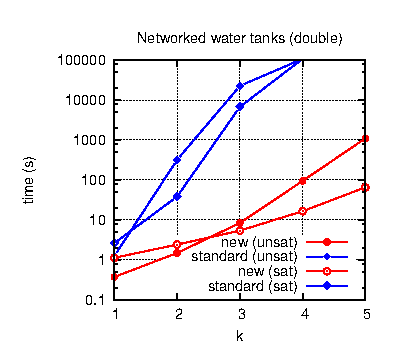
\includegraphics[width=0.45\columnwidth]{plot/water-double.eps}    
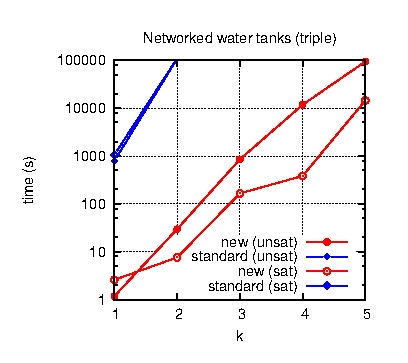
\includegraphics[width=0.45\columnwidth]{plot/water-triple.eps}    
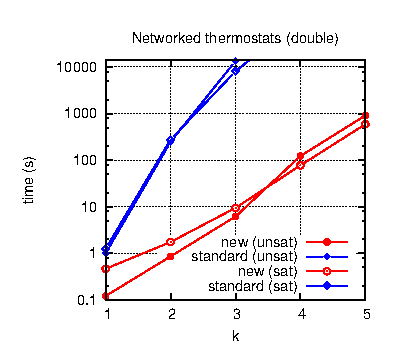
\includegraphics[width=0.45\columnwidth]{plot/thermostat-double.eps}    
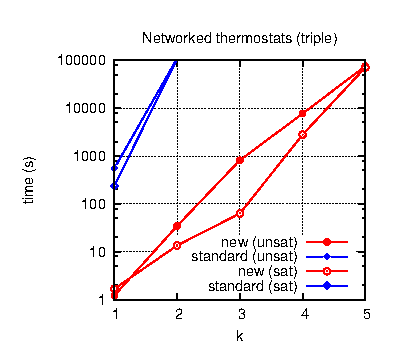
\includegraphics[width=0.45\columnwidth]{plot/thermostat-triple.eps}    
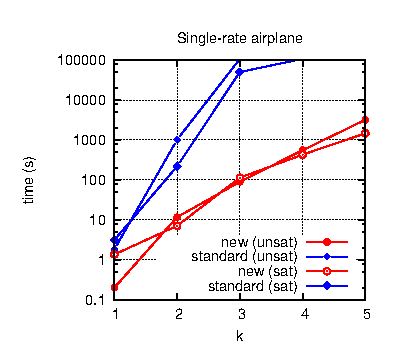
\includegraphics[width=0.45\columnwidth]{plot/airplane-single.eps}    
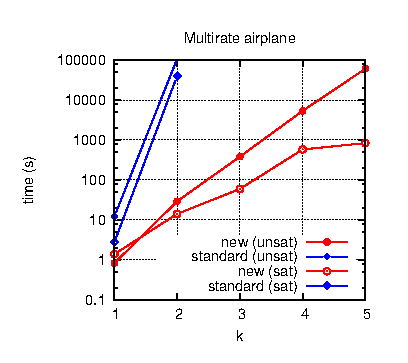
\includegraphics[width=0.45\columnwidth]{plot/airplane-multi.eps}    
\caption{Running time of $k$-step bounded model checking}
\label{table:bounded}
\end{figure}


